\documentclass[11pt]{article}
    \usepackage{comment} % enables the use of multi-line comments (\ifx \fi) 
    \usepackage{lipsum} %This package just generates Lorem Ipsum filler text. 
    \usepackage{fullpage} % changes the margin
    % Used for importing figures
    \usepackage{graphicx}
    \usepackage{wrapfig}
    \usepackage{float}
    \usepackage{subcaption}
    
\begin{document}

%Header-Make sure you update this information!!!!
\noindent
\large\textbf{Lab 2} \hfill \textbf{Zach Colbert} \\
\normalsize PH 411 \hfill Lab Partner: Michael Trumbull \\
Electronics  \hfill Due Date: 17 Oct 2017\\

\section{Thevenin Equivalent Potential and Resistance}
\subsection{Introduction}
    Thevenin's Theorem says that any combination of voltage sources and resistors in a circuit with two terminals are equivalent to a circuit with a single ideal voltage source and single resistor in series. This kind of equivalent circuit can reduce complex electrical systems to a simple one, for which a broad range of calculations are a lot easier. \\

    In this part of the lab, we take two approaches to finding the Thevenin equivalent potential and resistance of circuits fitting the parameters of Thevenin's Theorem. First, statically with resistors and digital multimeters on a Thevenin circuit with no load; Second, with a potentiometer load and a current-potential characteristic. \\

\subsection{Experimental}
    The Thevenin equivalent potential has been shown to be the open circuit potential across two points \(A\) and \(B\). As a result, \(V_{Th}\) is easily measured with a digital multimeter across those two points in the circuit. \\
    
    % FIGURE: Original circuit and Thevenin equivalent
    % \begin{figure}[H]
    %     \centering
    %     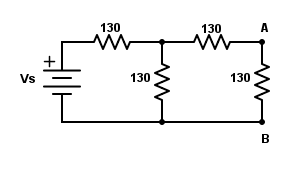
\includegraphics{1a_original.png}
    %     \caption{Original circuit.}
    %     \label{fig:1a_original}
    % \end{figure}

    % \begin{figure}[H]
    %     \centering
    %     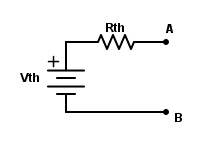
\includegraphics{1a_thevenin.png}
    %     \caption{Thevenin equivalent of \ref{fig:1a_original}}
    %     \label{fig:1a_thevenin}
    % \end{figure}

    \begin{figure}[H]
        \centering
        \begin{subfigure}{0.4\textwidth}
            \centering
            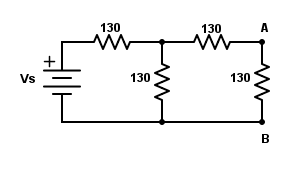
\includegraphics[width=\textwidth]{1a_original.png}
            \caption{The original circuit.}
            \label{fig:1a_original}
        \end{subfigure}
        %
        \begin{subfigure}{0.4\textwidth}
            \centering
            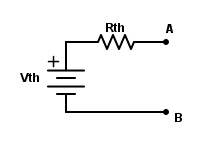
\includegraphics[width=\textwidth]{1a_thevenin.png}
            \caption{Thevenin equivalent of Figure \ref{fig:1a_original}}
            \label{fig:1a_thevenin}
        \end{subfigure}
        \caption{The given circuit and it's Thevenin equivalent circuit.}
    \end{figure}

    Assuming the DMM acts as an ideal voltmeter (with infinite resistance so no current passes through it), we know that the Thevenin resistance \(R_{Th}\) can be calculated by \\

    % FORMULA: Rth = Vth / Isc
    \begin{equation}
        \label{eqn:thevenin}
        R_{Th} = \frac{V_{Th}}{I_{SC}}
    \end{equation} \\

    where \(I_{SC}\) is the current through a short circuit between points \(A\) and \(B\). Again, assuming that the DMM acts as an ideal ammeter (with zero resistance so there is no potential difference across it), we use it to create a short circuit between \(A\) and \(B\) and measure the current. \\

    Our second method involves a slightly altered version of this circuit, with an additional potentiometer acting as a load resistor. \\

    % FIGURE: Circuit with load and Thevenin equivalent with load
    % \begin{figure}[H]
    %     \centering
    %     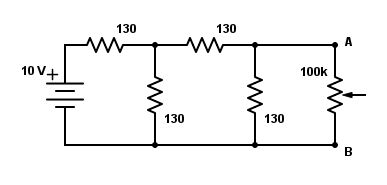
\includegraphics{1d_originalLoad.png}
    %     \caption{Original circuit \ref{fig:1a_original} with variable resistor load.}
    %     \label{fig:1d_originalLoad}
    % \end{figure}

    % \begin{figure}[H]
    %     \centering
    %     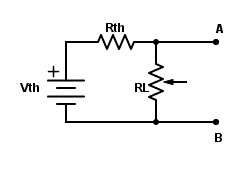
\includegraphics{1d_theveninLoad.png}
    %     \caption{Thevenin equivalent of \ref{fig:1a_original} with variable resistor load.}
    %     \label{fig:1d_theveninLoad}
    % \end{figure}

    \begin{figure}[H]
        \centering
        \begin{subfigure}{0.5\textwidth}
            \centering
            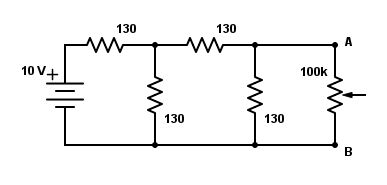
\includegraphics[width=\textwidth]{1d_originalLoad.png}
            \caption{Original circuit \ref{fig:1a_original} with variable resistor load.}
            \label{fig:1d_originalLoad}
        \end{subfigure}
        %
        \begin{subfigure}{0.3\textwidth}
            \centering
            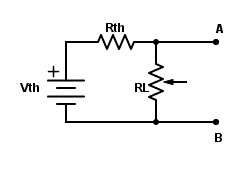
\includegraphics[width=\textwidth]{1d_theveninLoad.png}
            \caption{Thevenin equivalent of \ref{fig:1a_original} with variable resistor load.}
            \label{fig:1d_theveninLoad}
        \end{subfigure}
        \caption{The circuit with a variable resistor load, and it's Thevenin equivalent circuit.}
    \end{figure}

    In this case, the equation relating our desired values is a little more complex, but can still be represented as a linear function. \\

    % FORMULA: I = (Vth / Rth) - (1 / Rth) * Vab
    \begin{equation}
        \label{eqn:theveninLoad}
        I = \frac{V_{Th}}{R_{Th}} - \frac{1}{R_{Th}} V_{AB}
    \end{equation} \\
    
    Fundamentally, what we see is a current-potential characteristic with some particular features. Notably, where \(V_{AB} = 0\) we find that \(I = V_{Th} / R_{Th}\) (no potential difference implies no load resistance, and therefore a short circuit); and where \(I = 0\) we find that \(V_{Th} = V_{AB}\) (no current implies infinite load resistance, or an open circuit). \\

\subsection{Results}
    In Part 1, we used a source voltage \(V_s\) of \(10.0 V\). Using our first method, we measured \(V_{AB} = V_{Th}\) of \(2.00 V\) and \(I_{SC}\) of \(25.8 mA\). By Equation \ref{eqn:thevenin}, we calculated an \(R_{Th}\) of \(77.5 \Omega\). \\
    
    \begin{figure}[H]
        \centering
        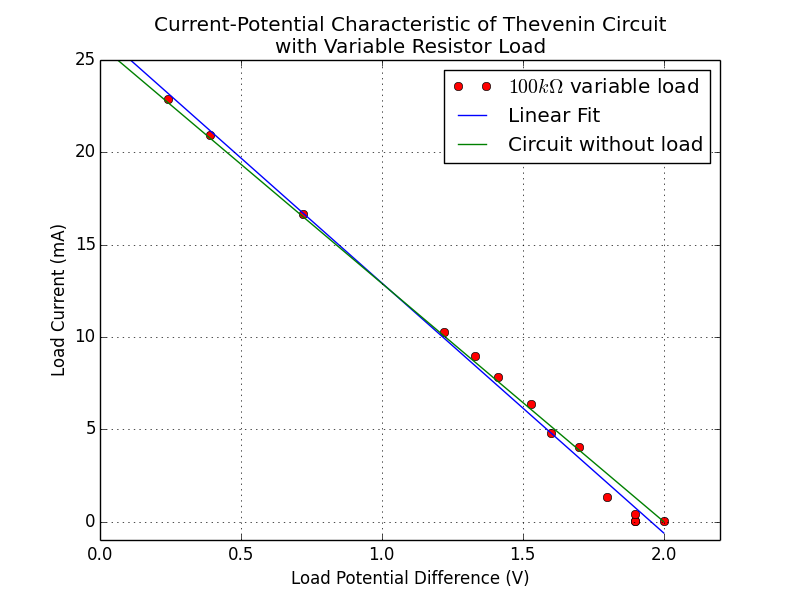
\includegraphics[width=0.8\textwidth]{fig_TheveninWithLoad.png}
        \caption{Results of the second method show a linear current-potential characteristic for the Thevenin equivalent circuit with variable resistor load.}
        \label{fig:fig_TheveninWithLoad}
    \end{figure}

    Our second method, measuring the circuit with \(100 k\Omega\) variable load, returned some very similar results as seen in Figure \ref{fig:fig_TheveninWithLoad}. The linear fit of our data shows a Thevenin resistance of \(73.86 \Omega\) and a Thevenin potential of \(1.95 V\). \\
    
    For comparison, we can find the values of \(V_{Th}\) and \(R_{Th}\) by using Kirchoff's Laws with the original circuit. By solving Equations \ref{kirchoff1}--\ref{kirchoff3} we find that the expected value of \(V_{Th}\) is \(2 V\), consistent with our earlier results. \\
    
    % FORMULA: Kirchoff rules for the original circuit
    \begin{equation}
        \label{kirchoff1}
        I_1 = I_2 + I_3
    \end{equation}
    \begin{equation}
        \label{kirchoff2}
        0 = 10V - 130 I_1 - 130 I_2       
    \end{equation}
    \begin{equation}
        \label{kirchoff3}
        0 = 130 I_2 - 130 I_3 - 130 I_3        
    \end{equation} \\

    It's important to note for this part that calculating the voltage is very straightforward using loop and junction rules, but when simplifying the circuit down to its Thevenin equivalent to find \(R_{Th}\) we need to short the source voltage and start to consider the resistors relative to the points \(A\) and \(B\). \\

    % FIGURES: Simplifying circuit to Thevenin equivalent
    % \begin{figure}[H]
    %     \centering
    %     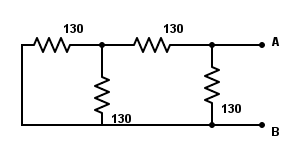
\includegraphics{1_simplify1.png}
    %     \caption{The original circuit \ref{fig:1a_original} with the voltage source shorted out.}
    %     \label{fig:1_simplify1}
    % \end{figure}

    % \begin{figure}[H]
    %     \centering
    %     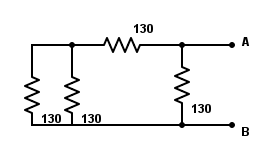
\includegraphics{1_simplify2.png}
    %     \caption{Relative to the points \(A\) and \(B\), the leftmost resistors are now parallel.}
    %     \label{fig:1_simplify2}
    % \end{figure}

    % \begin{figure}[H]
    %     \centering
    %     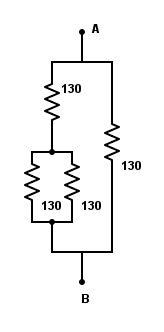
\includegraphics{1_simplify3.png}
    %     \caption{By rearranging the elements in the circuit, it's easier to tell which resistors are in parallel and which are in series. Here, it's plain to see that the resistors can reduce to an equivalent resistance of \(78 \Omega\).}
    %     \label{fig:1_simplify3}
    % \end{figure}

    \begin{figure}[H]
        \centering
        \begin{subfigure}{0.3\textwidth}
            \centering
            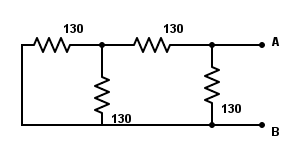
\includegraphics[width=\textwidth]{1_simplify1.png}
            % \caption{The original circuit \ref{fig:1a_original} with the voltage source shorted out.}
            \caption{}
            \label{fig:1_simplify1}
        \end{subfigure}
        %
        \begin{subfigure}{0.3\textwidth}
            \centering
            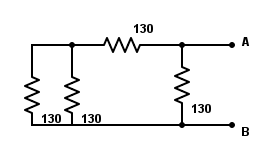
\includegraphics[width=\textwidth]{1_simplify2.png}
            % \caption{Relative to the points \(A\) and \(B\), the leftmost resistors are now parallel.}
            \caption{}
            \label{fig:1_simplify2}
        \end{subfigure}
        %
        \begin{subfigure}{0.3\textwidth}
            \centering
            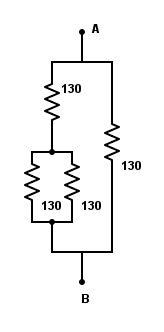
\includegraphics[width=\textwidth]{1_simplify3.png}
            \caption{}
            \label{fig:1_simplify3}
        \end{subfigure}
        \caption{By rearranging the elements in the circuit relative to the points $A$ and $B$, it's easier to tell which resistors are in parallel and which are in series.}
    \end{figure}

    Figures \ref{fig:1_simplify1} through \ref{fig:1_simplify3} demonstrate how to simplify the circuit to find the Thevenin resistance $R_{Th}$. This is different than simple equivalent circuit because Thevenin's Theorem requires us to short circuit (or remove, effectively) the voltage source from the circuit. When we do that, and look at the resistors relative to the points $A$ and $B$, elements that we may have seen in series with each other before are now in parallel.

    Consistent with our earlier results, we find the expected value of \(R_{Th}\) is \(78 \Omega\). \\

\subsection{Conclusion}
    The Thevenin equivalent of a circuit can be useful in cutting down time and mistakes making complex calculations, and reliable in that it gives us results consistent with what we expect from traditional calculations based on Kirchoff's Laws. \\
    
    As seen above, our results from both methods of finding the Thevenin potential and resistance are very close to the expected theoretical value. It was interesting to find that the first method (which I expected to be less accurate because it relies on only a single set of measurements and calculations) seems to be closer to the theoretical values than the second method (which relies on a larger sample, but allows more room for error in calculations). \\
    
    Ultimately, both methods result in Thevenin values very close to the theoretical values--the worst coming in a little over 5\% error. That seems like an acceptable margin for most applications, especially considering we did not put much effort in to mitigate error in measurement or calculations.\\
    
%%% PART 2 %%%

\section{Source and Input Resistances}
\subsection{Introduction}
    As was demonstrated in Part 1, Thevenin's Theorem provides a method for reducing complex circuits to simple ones. By an extension of that idea, we can use similar methods to simplify unknown circuits and describe them with just the Thevenin potential and resistance values. \\
    
    In Part 2, we use a variable resistor load and a current-potential curve (as in the second method of Part 1) to define the Thevenin equivalent circuits for a lab DC power supply and digital multimeter. \\
    
\subsection{Experimental}
    The applicable circuit diagrams are given in the lab assignment.
    In the case of the DC power supply, we consider the power supply to be the entire Thevenin circuit. Just as in Part 1, we used a variable resistor load and measured the potential difference across it and current through it. We reuse Equation \ref{eqn:theveninLoad} from above, with a couple of variables renamed: \\
    
    % FORMULA: I = (Voc / Rout) - (1 / Rout) * Vab
    \begin{equation}
        \label{eqn:theveninLoad_alt}
        I = \frac{V_{oc}}{R_{out}} - \frac{1}{R_{out}} V_{AB}
    \end{equation} \\

    In the case of the digital multimeter, the circuit looks a little different but is effectively the same as a simple Thevenin circuit with no load. Because $V_{AB}$ is inside of the DMM in this case, we choose to hold the power supply voltage $V_{in}$ constant and vary the load resistance so that we can use the equality between the current through the circuit, the potential difference measured by the DMM, and the internal resistance of the DMM. \\
    
    % FORMULA: I = Vab / Rin
    \begin{equation}
        \label{eqn:thevenin_alt}
        I = \frac{V_{AB}}{R_{in}}        
    \end{equation} \\

\subsection{Results}
    For the first case, we chose a \(10 \Omega\) variable resistor as our load and set a constant source voltage of \(1 V\) from the power supply. The current-potential characteristic and a linear fit based on Equation \ref{eqn:theveninLoad_alt} show that the output resistance \(R_{out}\) of the power supply is about \(1.77 \Omega\). \\
    
    % FIGURE: fig_PowerSupply
    \begin{figure}[H]
        \centering
        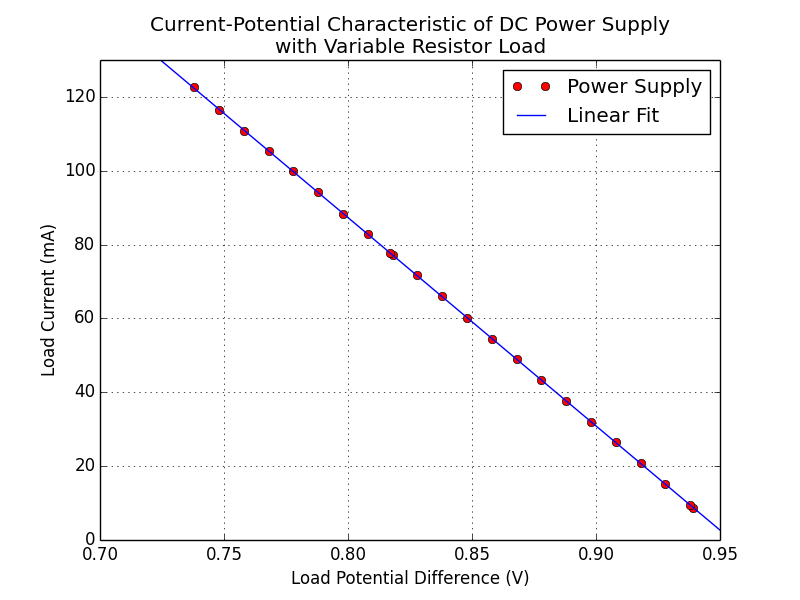
\includegraphics[width=\textwidth]{fig_PowerSupply.png}
        \caption{The current-potential characteristic of the power supply with variable resistor load.}
        \label{fig:powerSupply}
    \end{figure}

    For the second case, the calculations are simple enough that we don't need a characteristic curve. Instead, it's sufficient to find the average input resistance \(R_{in}\) over a few values for current and potential.\\

    % TABLE: 2b results
    \begin{center}
        \begin{tabular}{ |c|c|c| }
            \( V_{AB} \) & \( I (\mu A) \) & \( R_{in} (M\Omega) \) \\
            \hline
            8.9 & 0.9 & 9.9 \\
            \hline
            4.8 & 0.5 & 9.6 \\
            \hline
            3.2 & 0.3 & 10.7 \\
            \hline
            \hline
            & Average \( R_{in} \) & 10.1
        \end{tabular}
    \end{center}

    For the DMM, we find the input resistance to be $10.1 M\Omega$. \\

\subsection{Conclusion}
    The results from both cases are on the order of what we’d expect from the devices we’re testing--for a DC power supply, we expect a very small internal resistance so that it doesn’t affect the current through the attached circuit. For a voltmeter (the mode we operated our DMM in), we expect a very large resistance so that nearly all of the current in the circuit remains in the circuit. \\
    
    For circuits sensitive to the internal resistance of these devices, we’ve shown that Thevenin’s Theorem and the methods associated with it can make it relatively easy to determine the internal resistance of a device. 

\end{document}
